	\begin{figure}[H]
		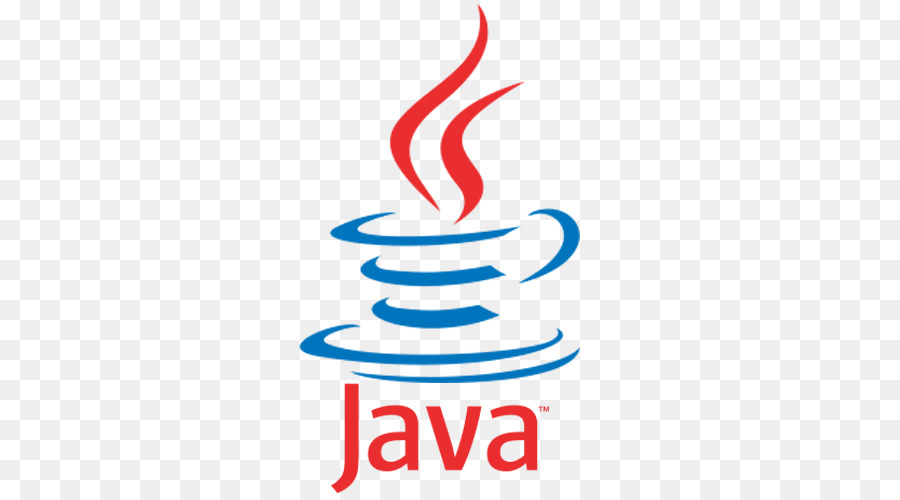
\includegraphics[width=6cm]{figures/web/javalogo.jpg}
		\centering
		\caption{Creator PHP Rasmus Lerdorf }
	\end{figure}
\subsection{Apa itu Java?}
Java adalah bahasa pemrograman yang dapat dijalankan di berbagai komputer termasuk telepon genggam. Bahasa ini awalnya dibuat oleh James Gosling saat masih bergabung di Sun Microsystems saat ini merupakan bagian dari Oracle dan dirilis tahun 1995. Bahasa ini banyak mengadopsi sintaksis yang terdapat pada C dan C++ namun dengan sintaksis model objek yang lebih sederhana serta dukungan rutin-rutin aras bawah yang minimal. Aplikasi-aplikasi berbasis java umumnya dikompilasi ke dalam p-code (bytecode) dan dapat dijalankan pada berbagai Mesin Virtual Java (JVM). Java merupakan bahasa pemrograman yang bersifat umum/non-spesifik (general purpose), dan secara khusus didisain untuk memanfaatkan dependensi implementasi seminimal mungkin. Karena fungsionalitasnya yang memungkinkan aplikasi java mampu berjalan di beberapa platform sistem operasi yang berbeda, java dikenal pula dengan slogannya, "Tulis sekali, jalankan di mana pun". Saat ini java merupakan bahasa pemrograman yang paling populer digunakan, dan secara luas dimanfaatkan dalam pengembangan berbagai jenis perangkat lunak aplikasi ataupun aplikasi.

\subsection{Sejarah Java}
Bahasa pemrograman Java terlahir dari The Green Project, yang berjalan selama 18 bulan, dari awal tahun 1991 hingga musim panas 1992. Proyek tersebut belum menggunakan versi yang dinamakan Oak. Proyek ini dimotori oleh Patrick Naughton, Mike Sheridan, dan James Gosling, beserta sembilan pemrogram lainnya dari Sun Microsystems. Salah satu hasil proyek ini adalah maskot Duke yang dibuat oleh Joe Palrang.

Pertemuan proyek berlangsung di sebuah gedung perkantoran Sand Hill Road di Menlo Park. Sekitar musim panas 1992 proyek ini ditutup dengan menghasilkan sebuah program Java Oak pertama, yang ditujukan sebagai pengendali sebuah peralatan dengan teknologi layar sentuh (touch screen), seperti pada PDA sekarang ini. Teknologi baru ini dinamai "*7" (Star Seven).

Setelah era Star Seven selesai, sebuah anak perusahaan Tv kabel tertarik ditambah beberapa orang dari proyek The Green Project. Mereka memusatkan kegiatannya pada sebuah ruangan kantor di 100 Hamilton Avenue, Palo Alto.

Perusahaan baru ini bertambah maju: jumlah karyawan meningkat dalam waktu singkat dari 13 menjadi 70 orang. Pada rentang waktu ini juga ditetapkan pemakaian Internet sebagai medium yang menjembatani kerja dan ide di antara mereka. Pada awal tahun 1990-an, Internet masih merupakan rintisan, yang dipakai hanya di kalangan akademisi dan militer.

Mereka menjadikan perambah (browser) Mosaic sebagai landasan awal untuk membuat perambah Java pertama yang dinamai Web Runner, terinsipirasi dari film 1980-an, Blade Runner. Pada perkembangan rilis pertama, Web Runner berganti nama menjadi Hot Java.

Pada sekitar bulan Maret 1995, untuk pertama kali kode sumber Java versi 1.0a2 dibuka. Kesuksesan mereka diikuti dengan untuk pemberitaan pertama kali pada surat kabar San Jose Mercury News pada tanggal 23 Mei 1995.

Sayang terjadi perpecahan di antara mereka suatu hari pada pukul 04.00 di sebuah ruangan hotel Sheraton Palace. Tiga dari pimpinan utama proyek, Eric Schmidt dan George Paolini dari Sun Microsystems bersama Marc Andreessen, membentuk Netscape.

Nama Oak, diambil dari pohon oak yang tumbuh di depan jendela ruangan kerja "Bapak Java", James Gosling. Nama Oak ini tidak dipakai untuk versi release Java karena sebuah perangkat lunak lain sudah terdaftar dengan merek dagang tersebut, sehingga diambil nama penggantinya menjadi "Java". Nama ini diambil dari kopi murni yang digiling langsung dari biji (kopi tubruk) kesukaan Gosling. Konon kopi ini berasal dari Pulau Jawa. Jadi nama bahasa pemrograman Java tidak lain berasal dari kata Jawa (bahasa Inggris untuk Jawa adalah Java).

\subsection{Kelebihan Java}
\begin{enumerate}
	\item Multiplatform. Kelebihan utama dari Java ialah dapat dijalankan di beberapa platform / sistem operasi komputer, sesuai dengan prinsip tulis sekali, jalankan di mana saja. Dengan kelebihan ini pemrogram cukup menulis sebuah program Java dan dikompilasi (diubah, dari bahasa yang dimengerti manusia menjadi bahasa mesin / bytecode) sekali lalu hasilnya dapat dijalankan di atas beberapa platform tanpa perubahan. Kelebihan ini memungkinkan sebuah program berbasis java dikerjakan di atas operating system Linux tetapi dijalankan dengan baik di atas Microsoft Windows. Platform yang didukung sampai saat ini adalah Microsoft Windows, Linux, Mac OS dan Sun Solaris. Penyebabnya adalah setiap sistem operasi menggunakan programnya sendiri-sendiri (yang dapat diunduh dari situs Java) untuk meninterpretasikan bytecode tersebut
	\item OOP (Object Oriented Programming - Pemrogram Berorientasi Objek), Java merupakan salah satu bahasa pemrograman dengan konsep OOP. Dimana program yang dibangun berorientasikan kepada Object. Aplikasi yang dibangun dengan konsep OOP terdiri atas object-object yang saling berhubungan
	\item Library yang lengkap, Java terkenal dengan kelengkapan library/perpustakaan (kumpulan program program yang disertakan dalam pemrograman java) yang sangat memudahkan dalam penggunaan oleh para pemrogram untuk membangun aplikasinya. Kelengkapan perpustakaan ini ditambah dengan keberadaan komunitas Java yang besar yang terus menerus membuat perpustakaan-perpustakaan baru untuk melingkupi seluruh kebutuhan pembangunan aplikasi.
	\item Garbage Colletor yang otomatis, memiliki fasilitas pengaturan penggunaan memori sehingga para pemrogram tidak perlu melakukan pengaturan memori secara langsung (seperti halnya dalam bahasa C++ yang dipakai secara luas).
	\item Simple, dibandingkan dengan bahasa pemrograman lain seperti C++
	\item Multithereaded, Java memiliki potensi untuk program berjalan secara multithreaded
	\item Aman
	\item Populer
	\item Komunitas yang mendukung
	\item Dokumentasi yang lengkap
\end{enumerate}

\subsection{Kekurangan Java}
\begin{enumerate}
	\item Mudah didekompilasi. Dekompilasi adalah proses membalikkan dari kode jadi menjadi kode sumber. Ini dimungkinkan karena kode jadi Java merupakan bytecode yang menyimpan banyak atribut bahasa tingkat tinggi, seperti nama-nama kelas, metode, dan tipe data. Hal yang sama juga terjadi pada Microsoft .NET Platform. Dengan demikian, algoritma yang digunakan program akan lebih sulit disembunyikan dan mudah dibajak/direverse-engineer.
	\item Penggunaan memori yang banyak. Penggunaan memori untuk program berbasis Java jauh lebih besar daripada bahasa tingkat tinggi generasi sebelumnya seperti C/C++ dan Pascal (lebih spesifik lagi, Delphi dan Object Pascal). Biasanya ini bukan merupakan masalah bagi pihak yang menggunakan teknologi terbaru (karena trend memori terpasang makin murah), tetapi menjadi masalah bagi mereka yang masih harus berkutat dengan mesin komputer berumur lebih dari 4 tahun
	\item Perfomance, Bahasa Java berjalan lebih lembat dibandingkan dengan bahasa lain
\end{enumerate}

\subsection{Contoh Kode Java Hello World}
	\begin{figure}[H]
		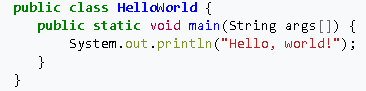
\includegraphics[width=6cm]{figures/web/contohjava.png}
		\centering
		\caption{Logo PHP}
	\end{figure}

\subsection{IDE (Integrated Development Environment) untuk Java}

\begin{enumerate}
	\item Netbeans
	\item Eclipse
	\item IntelliJ IDEA
\end{enumerate}
	\begin{figure}[H]
		
\includegraphics[width=6cm]{figures/android.jpg}
		\centering
		\caption{Logo Android}
	\end{figure}
\subsection{Apa itu Android?}
Android merupakan salah satu sistem operasi berbasis linux yang digunakan untuk perangkat ponsel pintar atau tablet yang dibuat dengan menggunakan bahasa pemrograman C, C++ dan juga Java. Android sendiri dibuat oleh perusahaan Android, Inc., yang kemudian google membelinya pada tahun 2005. Android resmi debut pada tahun 2007, tetapi ponsel pertama dengan sistem android baru pertama kali rilis satu tahun setelahnya yaitu pada tahun 2008. Android adalah sistem operasi open source yang dirilis oleh google dengan menggunakan lisensi apache, dengan terbukanya android untuk siapa saja memungkinkan untuk dilakukannya modifikasi secara bebas oleh siapapun yang membuat android pada oktober 2013 saja sudah memiliki 1 juta aplikasi yang ada pada playstore, dan juga suatu survey menyatakan bahwa android sangat populer di komunitas pengembang, sebanyak 71\%. Dan pada tahun 2014 saja sudah terdapat 1 milliar pengguna yang menggunakan android.

Hal-hal seperti inilah yang membuat android menjadi sistem operasi telepon pintar yang paling banyak digunakan di dunia dan dapat mengalahkan sistem operasi Symbian pada tahun 2010. Android juga menjadi pilihan banyak perusahaan karena berbiaya rendah, dapat dimodifikasi sesuai kebutuhan dan juga ringan, sifatnya yang open source juga menjadikan android memiliki banyak komunitas pengembang aplikasi yang menggunakan android untuk mengembangkan aplikasinya.

\subsection{Sejarah Android}
Android dibuat oleh perusahaan Android Inc. di Palo Alto, California pada oktober 2003 oleh seorang bernama Andy Rubin, RIch Miner, Nick Sears, dan juga Chris White, Android merupakan suatu projek yang memiliki banyak potensi dalam mengembangkan perangkat mobile yang sadar akan lokasi dan kesukaan pemiliknya. Awalnya, Android ini dikembangkan hanya untuk kamera digital, Kemudian perusahaan memutuskan bahwa pasar untuk kamera digital tidak terlalu besar untuk pencapaian yang diinginkan dan 5 bulan kemudian android dialihkan untuk dijadikan sebagai sistem operasi mobile yang akan menghadapi Symbian dan juga Windows Mobile.

Prototype awal ponsel pintar android sendiri awalnya mirip seperti ponsel Blackberry tanpa layer sentuh dan mempunyai keyboard qwerty, tetapi ketika Apple Iphone melakukan debutnya pada tahun 2007, Android terpaksa ditarik kembali ke tahap design dan akhirnya android juga mendukung layar sentuh tetapi tetap mendukung juga penggunaan keyboard qwerty tetapi pada akhirnya berfokus lebih ke layar sentuh. Ponsel pintar pertama yang menggunakan sistem operasi android secara komersial adalah HTC-Dream yang dikenal juga dengan nama T-Mobile G1 yang diumumkan pada 3 September 2003.
	\begin{figure}[H]
		
\includegraphics[width=6cm]{figures/AndroidStudio.jpg}
		\centering
		\caption{Android Studio}
	\end{figure}
\subsection{Mengenal Android Studio}
Android Studio adalah IDE pemrograman Android resmi dari Google yang dikembangkan dari IntelliJ. Sebelum ada Android Studio, programmer Android telah menggunakan Eclipse. Eclipse adalah IDE pemrograman Android sebelum munculnya Android Studio. Bisa dibilang Google telah berpaling dari Eclipse dan menjadikan Android Studio sebagai IDE resminya. Dikarenakan sudah meresmikan Android Studio pada tanggal 16 Mei 2013, Google menghentikan support ADT ke Eclipse tak lama kemudian dan ADT resmi hanya didapatkan oleh Android Studio.

Dikembangkan di atas IntelliJ IDEA besutan JetBrains, Android Studio dirancang khusus untuk pengembangan Android. IDE Ini tersedia untuk digunakan pada sistem operasi Windows, Mac OS X dan Linux.

\begin{figure}[H]
		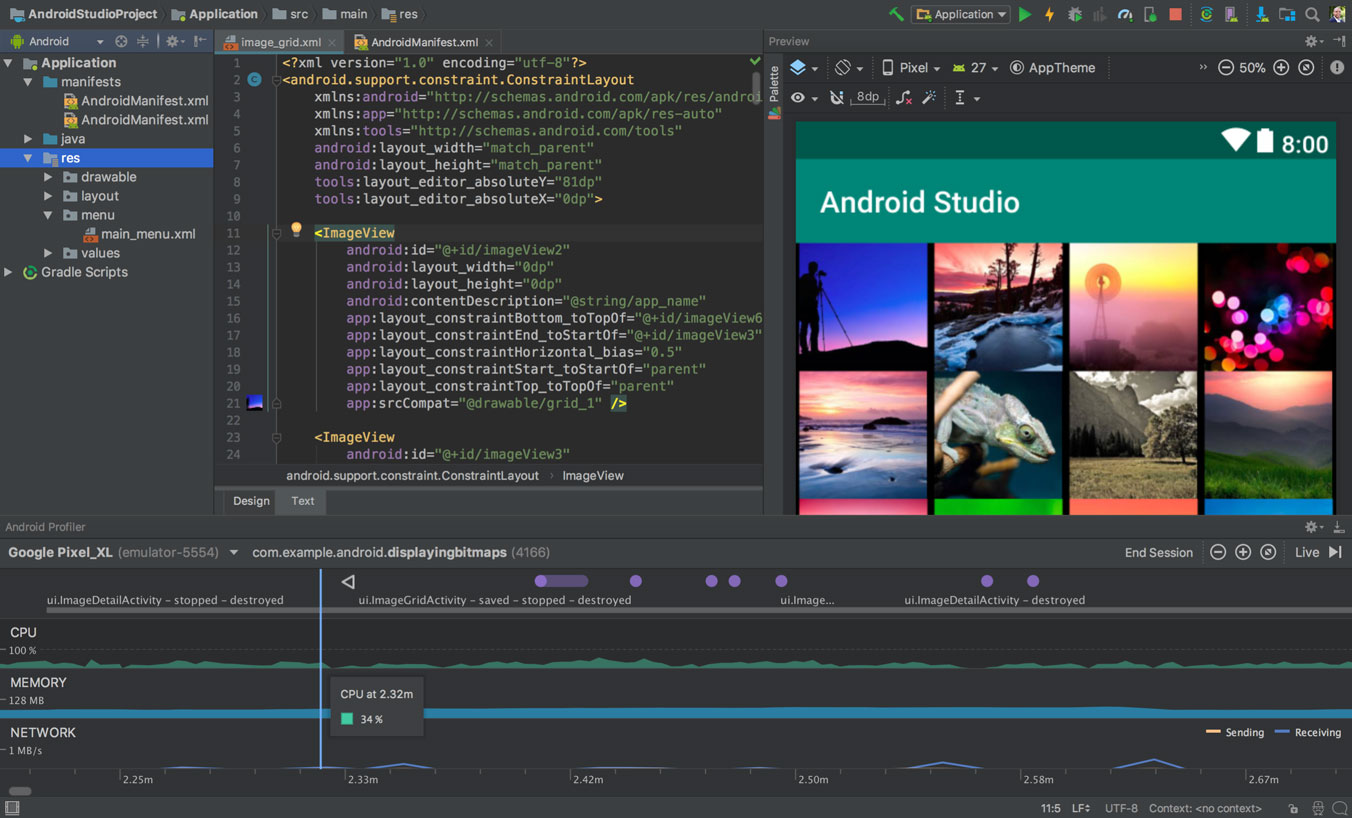
\includegraphics[width=6cm]{figures/tampilanandroidstudio.jpg}
		\centering
		\caption{Tampilan Android Studio}
	\end{figure}

\subsection{Mengapa Harus Android Studio}
\begin{enumerate}
	\item Gradle Build System
	\begin{enumerate}
		\item Android studion menggunakan sistem gradle yang terintegrasi yang digunakan untuk manajemen dependensi
		\item Membantu pengembang dalam mempermudah pengembangan karena gradle dapat dikembangkan dan dimodifikasi dengan mudah
	\end{enumerate}
	\item Ketersediaan drag and drop : Android Studio menyediakan Graphical User Interface sementara IDE seperti Eclipse tidak.
	\item User Interface : Android Studio lebih teroptimasi dalam hal tampilan dibandingkan dengan IDE lain seperti Eclipse terutama dalam mengembangkan aplikasi android.
	\item Java Code Auto-Completion : Meskipun IDE Eclipse juga memilikinya, tetapi versi di android studio lebih berjalan lancar dibandingkan dengan di Eclipse.
	\item Stability of System 
	\begin{enumerate}
		\item IDE Eclipse lebih besar dan lebih diutamakan untuk perangkat lunak berbasis java dibandingkan dengan Android Studio yang fokus untuk android.
		\item Android Studio lebih stabil karena memiliki lebih sedikit bug dibandingkand dengan Eclipse
		\item Spesifikasi Android Studio lebih rendah
	\end{enumerate}
\end{enumerate}

\subsection{Kelebihan dan Kekurangan dalam mengembangkan aplikasi Android}

Kelebihan
\begin{enumerate}
	\item Kemudahan dalam registrasi aplikasi : Dibandingkan dengan registrasi aplikasi ke Apple App Store, Google Playstore lebih mudah proses registrasinya, proses registrasi hanya membutuhkan waktu yang sebentar dan memiliki proses yang telah terotomatisasi tanpa pemerikasaan manual serta biaya registrasi yang lebih murah juga.
	\item Kebebasan Hardware : Android dikembangkan dengan menggunakan bahasa pemrograman java yang sangat mendukung terhadap cross-platform. Jadi anda bisa mengembangkan aplikasi android dari ataupun ke sistem operasi mana saja termasuk diantaranya adalah windows, mac os, ataupun linux. Sementara iOS sendiri hanya bisa di MAC atau di virtual machine.
	\item Java dan Kotlin sebagai bahasa pemrograman : Android mempunyai 2 bahasa yang didukung yaitu bahasa java dan juga kotlin. Java sudah dikenal dan terpecaya selama 2 dekade. Java merupakan bahasa yang berorientasi objek, cross-platform yang digunakan dimana saja dari web,dekstop,mobile, IoT dan lain lain. Sementara Kotlin sendiri lebih seperti ke cara yang lebih baik dalam menulis Java, Kotlin membuat penulisan kode menjadi lebih cepat, singkat dan mudah dibandingkan dengan java.
	\item Sumber pembelajaran : Tersedia dimana mana karena bahasa Java yang sudah dikenal dari dulu dan juga dukungan dari google-nya itu sendiri yang menyediakan dokumentasi dan training bagi mereka yang ingin belajar android.
	\item Lebih dari Mobile : Selain pengembangan android, android studio juga mendukung pengembangan dalam perangkat lain yaitu VR, Android TV, Wear OS, Android Auto, Android Things, dan juga Chrome OS devices, sehingga proses pembelajaran tidak berhenti di Mobile.
\end{enumerate}

Kekurangan
\begin{enumerate}
	\item Perilaku pengguna android : Beberapa survey menyatakan bahwa hanya sekitar 30 \% pengguna android yang melakukan transaksi di playstore dibandingkan dengan App Store, sebagai pengembang ini berarti pendapatan yang akan didapat dari playstore akan lebih sedikit dibandingkan jika anda menjadi developer untuk ponsel Iphone.
	\item Isu Keamanan : Open source memiliki keuntungan dan kerugiannya sendiri, dan kerugiannya itu adalah keamanan yang sering terjadi. Meskipun Google sering merilis update sekuriti, tetapi user terkadang sering mengabaikannya sehingga terkadang para pengembangnya sendiri yang harus menjaga data para penggunanya.
	\item Testing yang rumit : Testing yang rumit disebabkan karena masih banyaknya pengguna android yang menggunakan versi android versi lawas yang rilis tahun 2015,2016,2017 seperti Lolipop, marshmallow, dan Nougat.
	\item Kompatibilitas perangkat : Beberapa perusahaan yang memproduksi ponsel pintar memiliki spesifikasinya tersendiri dalam membuat produk, hal hal seperti besar layar, sensor, performa, dan juga driver yang berbeda beda menjadikan proses mengembangkan aplikasi android menjadi lebih sulit karena terkadang apa yang kita kembangkan tidak kompatibel dengan spesifikasi tertentu atau bisa juga karena teknologi yang dipakai masih baru sehingga kita terpaksa untuk menurunkan kualitas aplikasi.
	\item hak cipta : Dalam proses registrasi aplikasi untuk dipampang di playstore,  Google tidak mengecek hal-hal seperti hak cipta atau aplikasi ketiga yang kamu gunakan di aplikasi kamu, jadi terkadang kamu bisa juga terkena laporan pelanggaran hak cipta meskipun hal itu tidak disengaja.
\end{enumerate}
	\begin{figure}[H]
		
\includegraphics[width=6cm]{figures/web/php.png}
		\centering
		\caption{Logo PHP}
	\end{figure}
\subsection{Apa itu PHP?}
PHP merupakan salah satu dari sekian banyak bahasa pemrograman web yang paling umum digunakan dalam pengembangan suatu web. Biasanya dalam implementasinya PHP sering digabungkan atau disisipkan dalam dokumen HTML. PHP memiliki kepanjangan yaitu PHP: Hypertext Preprocessor.Bahasa pemrograman ini bersifat server-side. Arti dari Server-side programming sendiri yaitu script/program tersebut akan dijalankan/diproses oleh server. 

\subsection{Sejarah PHP}
Pada awalnya PHP merupakan kependekan dari Personal Home Page (Situs personal). PHP pertama kali dibuat oleh Rasmus Lerdorf pada tahun 1995. Pada waktu itu PHP masih bernama Form Interpreted (FI), yang wujudnya berupa sekumpulan skrip yang digunakan untuk mengolah data formulir dari web.

Selanjutnya Rasmus merilis kode sumber tersebut untuk umum dan menamakannya PHP/FI. Dengan perilisan kode sumber ini menjadi sumber terbuka, maka banyak pemrogram yang tertarik untuk ikut mengembangkan PHP.

Pada November 1997, dirilis PHP/FI 2.0. Pada rilis ini, interpreter PHP sudah diimplementasikan dalam program C. Dalam rilis ini disertakan juga modul-modul ekstensi yang meningkatkan kemampuan PHP/FI secara signifikan.

Pada tahun 1997, sebuah perusahaan bernama Zend menulis ulang interpreter PHP menjadi lebih bersih, lebih baik, dan lebih cepat. Kemudian pada Juni 1998, perusahaan tersebut merilis interpreter baru untuk PHP dan meresmikan rilis tersebut sebagai PHP 3.0 dan singkatan PHP diubah menjadi akronim berulang PHP: Hypertext Preprocessing.

Pada pertengahan tahun 1999, Zend merilis interpreter PHP baru dan rilis tersebut dikenal dengan PHP 4.0. PHP 4.0 adalah versi PHP yang paling banyak dipakai pada awal abad ke-21. Versi ini banyak dipakai disebabkan kemampuannya untuk membangun aplikasi web kompleks tetapi tetap memiliki kecepatan dan stabilitas yang tinggi.

Pada Juni 2004, Zend merilis PHP 5.0. Dalam versi ini, inti dari interpreter PHP mengalami perubahan besar. Versi ini juga memasukkan model pemrograman berorientasi objek ke dalam PHP untuk menjawab perkembangan bahasa pemrograman ke arah paradigma berorientasi objek. Peladen web bawaan ditambahkan pada versi 5.4 untuk mempermudah pengembang menjalankan kode PHP tanpa menginstal peladen perangkat lunak.

Versi terbaru dan stabil dari bahasa pemograman PHP saat ini adalah versi 7.4.3 yang dirilis pada tanggal 20 Februari 2020

\subsection{Sekilas tentang pembuat PHP : Rasmus Lerdorf}
	\begin{figure}[H]
		
\includegraphics[width=6cm]{figures/web/rasmuslerdorf.jpg}
		\centering
		\caption{Creator PHP Rasmus Lerdorf }
	\end{figure}
Rasmus Lerdorf merupakan seorang programmer yang berasal dari Denmark. Dia membuat dan membantu dalam hal pengkodean bahasa PHP, terutama pada 2 versi awal yang kemudian dikembangkan secara grup bersama dengan Jim Winstead (Yang membuat blo.gs), Stig Bakken, Shane Caraveo, Andi Gutmans, dan juga Zeev Suraski. sampai sekarang ia terus berkontribusi pada projek.

Lerdorf lahir di pulau disko di daerah Greenland dan kemudian pindah ke Denmark pada awal hidupnya. kelaurganya pindah dari Kanada ke Denmark pada tahun 1980, lalu pindah lagi ke kota King di Ontario pada tahun 1983. Dia lulus dari SMA King City pada tahun 1988, dan pada tahun 1993 lulus dari Universitas Waterloo dengan gelar  Bachelor of Applied Science di bidang teknik desain sistem. Dia juga ikut berkontribusi dalam Apache HTTP Server dan menambahkan clausa Limit pada mSQL DBMS. 

Dari Septermber 2002 sampai November 2009, Lerdorf bekerja di perusahaan Yahoo sebagai Infrastructure Architecture Engineer. Pada tahun 2010 kemudian bergabung ke perusahaan WePay untuk mengembangkan API (Application Programming Interface). dan pada tahun 2011 ia menjadi seorang konsultan untuk beberapa startup. Kemudian pada 22 Februari 2012 ia bergabung dengan Etsy, sebuah website e-commerce yang berfokus pada hal hal vintage. Dan pada tahun 2013, Rasmus bergabung dengan Jelastic sebagai Senior Advisor untuk membantu mereka mengembangkan teknologi baru.

Selain itu Lerdorf juga sering menjadi pembicara dalam konferensi open source di berbagai belahan dunia. Beberapa topik yang sering dia bahas diantaranya adalah security vulnerabilities dan juga tentang PHP.

Pada tahun 2003, ia di beri penghargaan oleh MIT Technology Review sebagai salah satu dari 100 inovator di dunia yang berada dibawah umur 35
\subsection{Website yang menggunakan PHP} 
	\begin{figure}[H]
		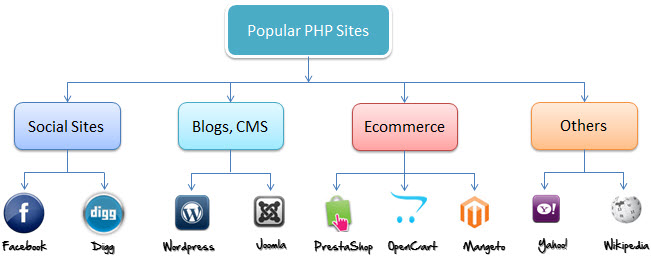
\includegraphics[width=8cm]{figures/web/popularphpsites.jpg}
		\centering
		\caption{Website dengan bahasa PHP}
	\end{figure}

\subsection{Contoh Kode PHP}
	\begin{figure}[H]
		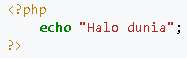
\includegraphics[width=6cm]{figures/web/contohkodingphp.png}
		\centering
		\caption{Program Hello world yang ditulis dengan PHP}
	\end{figure}

\subsection{Kelebihan PHP}
\begin{itemize}
	\item Bahasa Pemrograman PHP dapat ditemukan di mana - mana.
	\item Proses pengembangan lebih mudah, karena komunitas yang bisa dibilang besar dan mendukung.
	\item PHP adalah bahasa scripting yang paling mudah karena memiliki referensi yang banyak dan lengkap.
	\item PHP adalah bahasa open source yang dapat digunakan di berbagai mesin (Linux, Unix, Macintosh, Windows).
	\item Ringkas dan ringan
	\item Maintenanace Mudah
\end{itemize}
\subsection{Kekurangan PHP}
\begin{itemize}
	\item Banyak kompetisi, karena PHP adalah bahasa pemrograman yang paling umum
	\item Terkesan kurang prestigious.
	\item Tidak ideal jika untuk pengembangan skala besar.
	\item PHP mempunyai kelemahan security tertentu.
\end{itemize}

\subsection{Referensi belajar PHP}
\begin{itemize}
	\item php.net
	\item sitepoint.com
	\item tutorialspoint.com/php/
\end{itemize}

	\begin{figure}[H]
		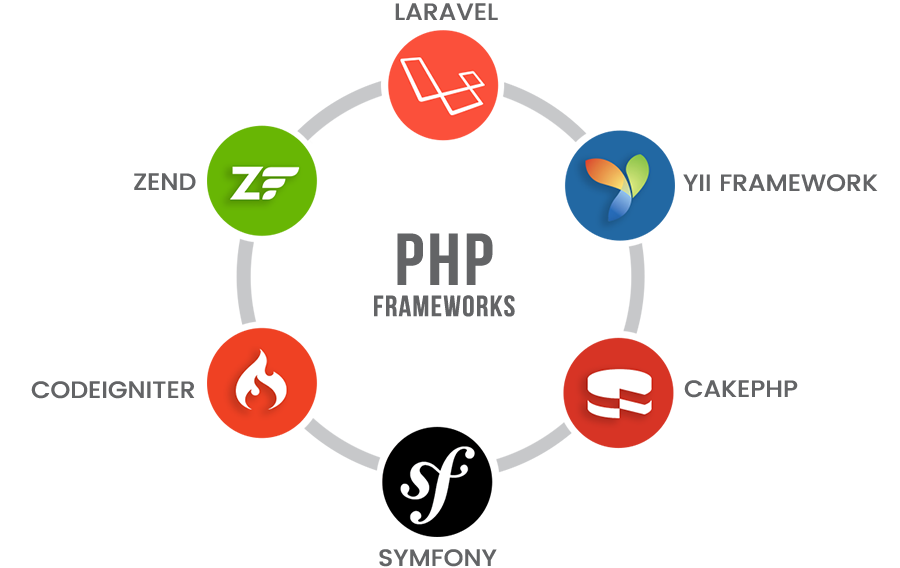
\includegraphics[width=12cm]{figures/web/phpframework.png}
		\centering
		\caption{Framework PHP}
	\end{figure}
\subsection{Apa itu Framework?}
PHP Framework adalah suatu kerangka keja yang telah terbentuk dan tersusun untuk memudahkan proses pengembangan website  secara profesional.

Namun perlu diketahui, bahwa PHP Framework memiliki perbedaannya tersendiri jika dibandingkan dengan sebuah CMS (Content Management System). Meskipun pada dasarnya mereka sama-sama memudahkan dalam hal yang sama yaitu pembuatan website. Tetapi untuk CMS  kita tidak perlu repot-repot dan pusing-pusing menulis script maupun sekumpulan kode. Dengan fitur CMS, semuanya telah dibuat instan dan kita hanya perlu sedikit mengatur bagian konten dan interface-nya saja.

Berbeda dengan Framework, kita tetap harus menuliskan script dan sekumpulan kode untuk dapat membangun sebuah web. 

\subsection{Mengapa harus menggunakan Framework?}
\begin{itemize}
	\item Mempercepat proses pengembangan web
	\item Kode yang terorganisir dan dapat digunakan terus menerus (reusable).
	\item Lebih mudah dalam proses maintenance.
	\item Lebih aman dalam hal sekuriti
	\item Menggunakan pola MVC (model - view - controller) yang memisahkan antara presentation dan logic
	\item Konsep web development modern seperti object oriented programming.

\end{itemize}

	\begin{figure}[H]
		
\includegraphics[width=6cm]{figures/web/logocodeigniter.png}
		\centering
		\caption{Logo Codeigniter}
	\end{figure}

\subsection{Pengenalan Codeigniter}

CodeIgniter sendiri merupakan salah satu framework php yang bersifat aplikasi sumber terbuka(Open Source) dengan model MVC (Model, View, Controller) yang digunakan untuk mengembangkan situs web yang dinamis. CodeIgniter mempermudah proses pengembang web untuk membuat aplikasi web dengan waktu yang lebih cepat dan mudah dibandingkan dengan membuatnya dari awal. CodeIgniter dirilis pertama kali pada 28 Februari 2006. 

	\begin{figure}[H]
		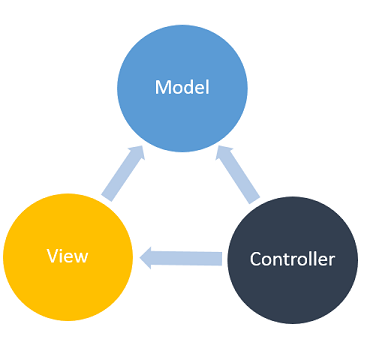
\includegraphics[width=8cm]{figures/web/mvc.png}
		\centering
		\caption{MVC Concept}
	\end{figure}
\subsection{Konsep MVC (Model View dan Controller)}
Model View Controller merupakan suatu konsep yang cukup populer dalam mengembangkan suatu aplikasi web, Konsep MVC ini mencoba memisahkan pengembangan aplikasi berdasarkan komponen-komponen utama dalam membuat suatu aplikasi seperti misalkan bagian untuk pemrosesan/manipulasi data, tampilan , dan bagian untuk kontrol aplikasi. Terdapat 3 jenis komponen yang membangun suatu pola MVC dalam suatu aplikasi yaitu: 
\begin{enumerate}
	\item View, merupakan bagian yang akan ditampilkan dan dilihat oleh pengguna. Biasanya, yang ditampilkan adalah dokumen HTML yang diatur oleh controller. View berfungsi untuk menerima dan merepresentasikan data kepada pengguna. Bagian view tidak dapat memiliki akses pada bagian model.
	\item Model, Berhubungan langsung dengan proses CRUD (Create, Read, Update, Delete), serta search. Model juga menangani validasi dari bagian controller, tetapi berhubungan langsung dengan view.
	\item Controller, merupakan bagian yang menghubungkan model dan juga view, controller berperan dalam menerima data dari view kemudian memprosesnya untuk dikirim ke bagian model.
\end{enumerate}

\subsection{Kelebihan dan Kekurangan Codeigniter}
\begin{itemize}
	\item Kelebihan
\begin{itemize}
	\item Performa sangat cepat.
	\item Konfigurasi yang sangat minim
	\item Komunitas yang aktif dan mendukung
	\item Dokumentasi yang sangat lengkap
\end{itemize}
	\item Kekurangan
\begin{itemize}
	\item CodeIgniter tidak ditujukan untuk pembuatan web dengan skala besar.
	\item Tidak Adanya Editor Khusus.
\end{itemize}
\end{itemize}
\subsection{Instalasi Codeigniter}
\begin{itemize}

	\begin{figure}[H]
		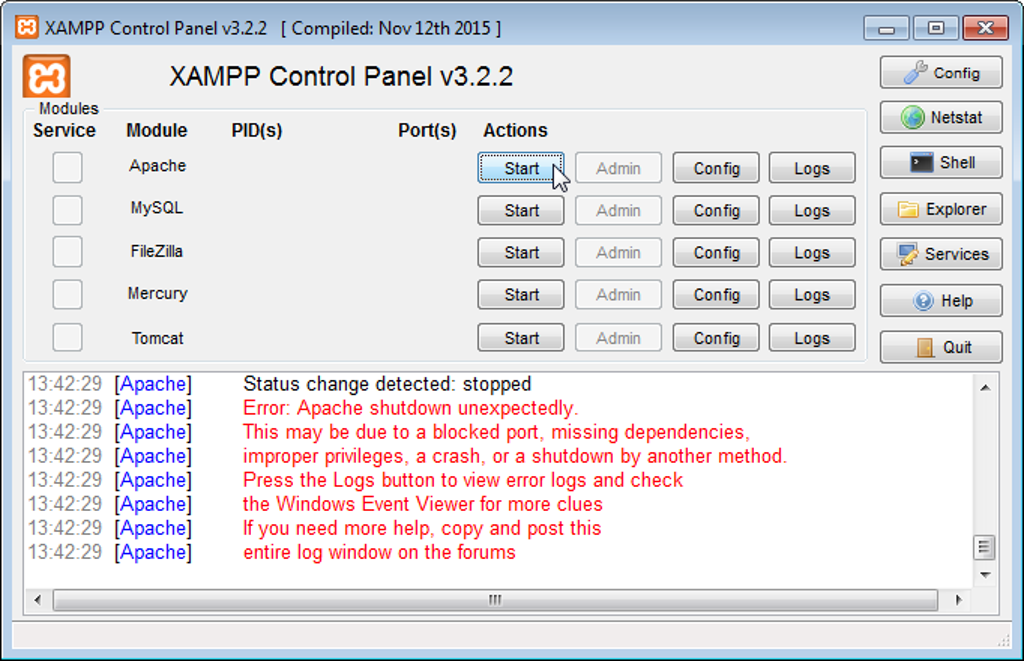
\includegraphics[width=8cm]{figures/web/Xampp.png}
		\centering
		\caption{Tampilan Xampp}
	\end{figure}
	\item Download Xampp terlebih dahulu di https://www.apachefriends.org/
	\item Kemudian install Xampp
	\begin{figure}[H]
		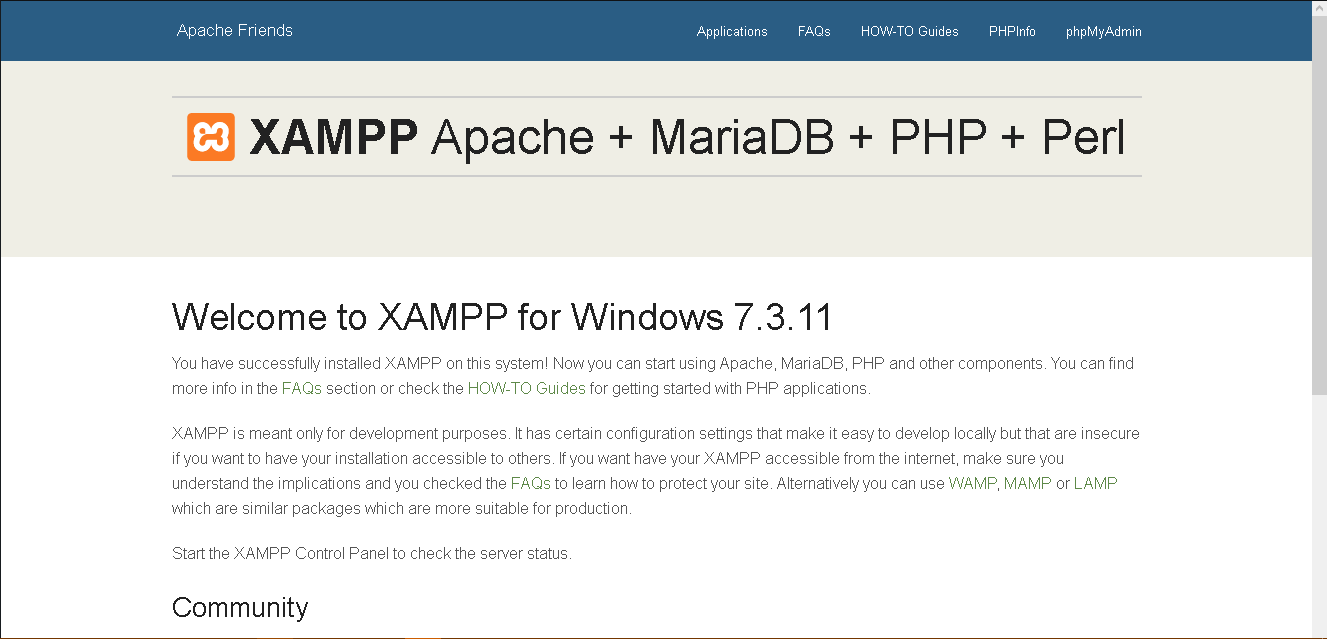
\includegraphics[width=8cm]{figures/web/tampilanwebxampp.png}
		\centering
		\caption{Tampilan web Xampp jika berhasil instalasi}
	\end{figure}


	\begin{figure}[H]
		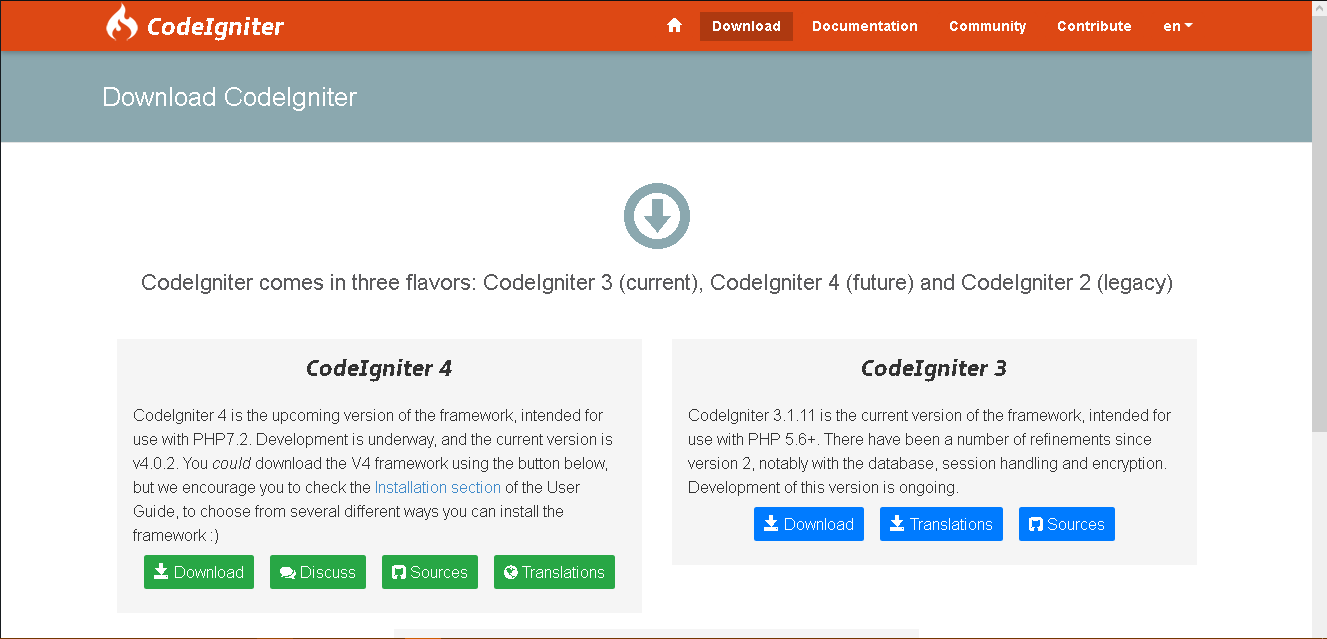
\includegraphics[width=8cm]{figures/web/websitecodeigniter.png}
		\centering
		\caption{Website Codeigniter}
	\end{figure}
	\item Kemudian, dilanjutkan dengan instalasi codeigniter dengan cara mendownload terlebih dahulu codeigniter-nya di https://codeigniter.com/en/download


	\begin{figure}[H]
		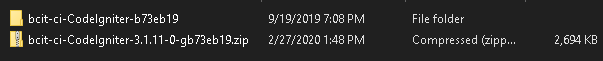
\includegraphics[width=8cm]{figures/web/ekstrakcodeigniter.png}
		\centering
		\caption{Ekstrak File}
	\end{figure}
	\item ekstrak file yang telah di download

	\item berikut adalah hasil ekstrak file
	\begin{figure}[H]
		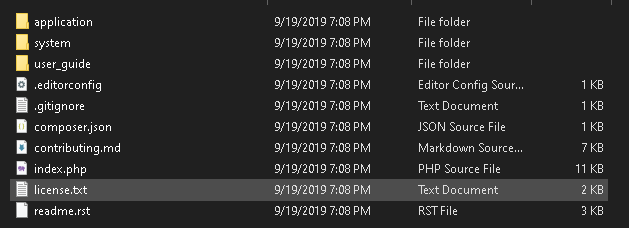
\includegraphics[width=8cm]{figures/web/hasilekstrakcodeigniter.png}
		\centering
		\caption{Hasil Ekstrak File}
	\end{figure}

\end{itemize}

	\begin{figure}[H]
		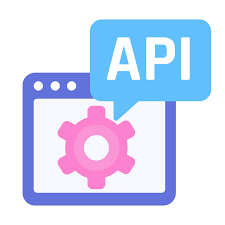
\includegraphics[width=8cm]{figures/GambarAPI.png}
		\centering
		\caption{API}
	\end{figure}
\subsection{Pengenalan API}
API merupakan kepanjangan dari Applicaiton Programming Interface. Sebuah API merupakan suatu software yang menjadi penengah diantara dua aplikasi yang berbeda supaya nantinya bisa berbicara atau berkomunikasi atau saling bertukar data satu sama lain. Artinya yaitu suatu API adalah pembawa pesan yang mengantarkan setiap permintaan kamu kepada penyedia layanan yang kamu inginkan kemudian mengantarkan kembali juga respon yang didapat dari layanan yang kamu inginkan kepada aplikasi yang sedang kamu gunakan.

API mendefinisikan suatu fungsionalitas yang independen berdasarkan implemntasinya masing masing, yang nantinya implementasi serta pendefinisiannya bisa berbeda-beda tanpa harus saling mengganggu satu sama lain. Oleh karena itu, suatu API yang bagus akan membuat proses pengembangan suatu program menjadi lebih mudah dengan cara menyediakan beberapa langkah cepat dalam mengembangkan suatu program.

Ketika seorang pengembang membuat kode, mereka tidak selalu mulai dari awal atau dari kosong. API membuat para pengembang ini mampu membuat kode yang kompleks dan bisa digunakan secara berulang dengan hanya mengetikan beberapa kode. Kecepatan dari API inilah yang membuat para pengembang menjadikan API sebagai hal yang krusial di setiap projek atau pengembangan suatu aplikasi.

Para pengembang sekarang sudah lebih produktif dibandingkan dengan dulu ketika mereka harus menulis berbagai macam kode dari awal. Dengan adanya API, sekarang mereka tidak harus mengulang semua proses dari awal atau mengetikan semuanya lagi secara berulang-ulang di setiap projekan baru. Sekarang para pengembang bisa lebih fokus terhadap permasalahan yang lain pada aplikasinya dan membiarkan API untuk menyelesaikan permasalahan umum yang sudah ada.
\subsection{Fungsi API}
API memiliki fungsi untuk menyediakan function yang lebih terstrukur serta terbaca dan mudah dipahami oleh seorang programmer. Hal ini merupakan hal yang krusial, terutama pada bagian editing serta pengembangan suatu projek

\subsection{Jenis-Jenis API}
\begin{enumerate}
	\item Ownership Web API
	\begin{enumerate}
		\item Open API : Open API adalah API tersedia untuk umum untuk digunakan seperti API Oauth dari Google dan tidak ada batasan untuk menggunakannya. Oleh karena itulah, mereka juga dikenal sebagai API Open atau Publik
		\item Partner API : Partner API adalah API dimana Hak atau Lisensi khusus untuk mengakses API jenis ini karena tidak tersedia untuk umum. Biasanya, API semacam ini dikaitkan dengan layanan berbayar.
		\item Internal API : API Internal adalah API yang dikembangkan oleh Perusahaan untuk digunakan ke dalam Sistem Internal mereka sehingga mereka dapat meningkatkan produktivitas tim pengembangan di mana satu tim dapat menggunakan layanan dari proyek lain perusahaan disebut API Internal. API ini juga dikenal sebagai API Pribadi.
		\item Composite API : Composite API, baik proses dan APIS komposit adalah urutan Task atau Tugas tetapi API Komposit atau Composite API menggabungkan Data dan API layanan yang berbeda. Ini adalah urutan Task atau Tugas yang berjalan secara sinkron sebagai hasil dari sebuah eksekusi, di mana hasil pemicu Composite API adalah hasil dari eksekusi dan bukan permintaan yang akan berisi hasil eksekusi atas Permintaan Task atau Tugas. Penggunaan utamanya adalah untuk mempercepat Proses Eksekusi dan meningkatkan kinerja pendengar di Antarmuka Web.
	\end{enumerate}
	\item Communication Level API
	\begin{enumerate}
		\item High Level API : High Level API adalah yang biasa kita gunakan secara umum dalam bentuk REST di mana Programmer memiliki tingkat abstraksi yang tinggi dan mereka hanya mementingkan melakukan Fungsi terbatas.
		\item Low Level API : Low Level API adalah API yang memiliki tingkat abstraksi yang lebih rendah sehingga lebih rinci, yang memungkinkan Programmer untuk memanipulasi Fungsi yang terdpat dalam Modul Aplikasi atau dalam Hardware (Perangkat Keras) pada tingkat granular. Biasanya, API Tingkat Rendah atau Low Level API ini digunakan dalam mengirim Video atau umpan Media Real-Time sebagai respons terhadap pemicu seperti Vulkan APIs.
	\end{enumerate}
	\item Web Service API : Dalam Web Service API, klasifikasinya dilakukan pada Jenis Komunikasi dan Pendekatan Behavior atau perilaku yang digunakan dalam membangun API seperti
	\begin{itemize}
		\item SOAP
		\item XML-RPC
		\item JSON-RPC
		\item REST
	\end{itemize}
\end{enumerate}


\begin{figure}[H]
		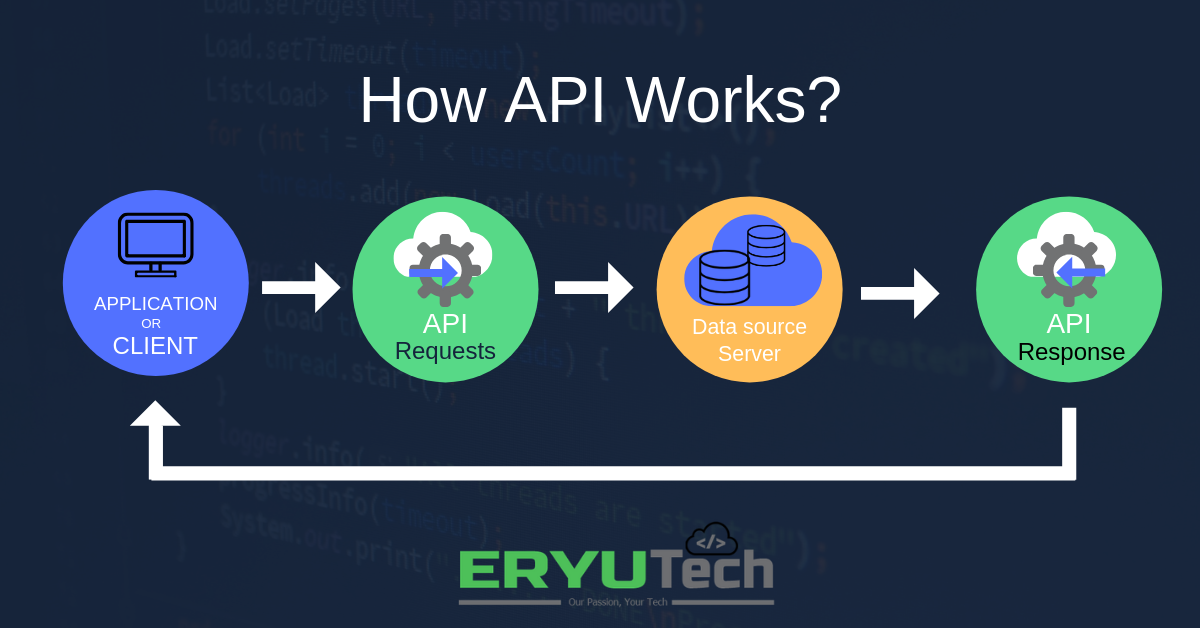
\includegraphics[width=8cm]{figures/carakerjaAPI.png}
		\centering
		\caption{Cara Kerja API}
	\end{figure}\subsection{Cara Kerja API}
Cara kerja API sendiri kurang lebih seperti bagaimana seorang pelayan restoran bekerja. anda sebagai customer yang sedang duduk di meja dengan menu untuk memilih pesanan anda, dan juga dapur sebagai penyedia dari apa yang anda inginkan.

Anda pasti butuh sesuatu yang menghubungkan pesanan anda dengan dapur restoran yang kemudian nanti akan diantarkan kembali ke meja anda. Pastinya itu tidak bisa seorang juru masak yang melakukannya karena ia perlu memasak di dapur. anda butuh sesuatu yang menghubungkan pelanggan yang sedang memesan suatu pesanan makanan dengan seorang juru masak yang akan mempersiapkan hal tersebut. nah disinilah seorang pelayan atau waiter atau bisa disebut juga sebagai API.

Pelayan atau bisa juga kita sebut sebagai API ini akan melayani pesanan anda dan mengantarkannya kebagian dapur untuk meminta dapur membuatkan pesanan anda yang kemudian akan di respon oleh dapur dalam hal ini yaitu makanan kembali ke anda.

\subsection{Contoh nyata API}
Bagaimana contoh implementasi nyata dari API itu sendiri? mungkin kamu pernah melihat atau mencoba memesan tiket pesawat?

Ketika kamu mencari jadwal penerbangan secara onine, kamu akan disajikan dengan menu dan opsi untuk dipilih. Kamu kemudian akan memilih kota keberangkatan dan juga tanggalnya serta destinasi beserta tanggal sampai, class kabinnya(ekonomi atau bisnis), atau hal-hal lain seperti misalkan makanan dan juga tempat duduk ataupun tempat untuk menyimpan bawaan.

Untuk melakukan proses booking penerbangan, kamu butuh untuk berinteraksi dengan website maskapai penerbangan untuk mengakses database maskapai untuk melihat apakah masih ada kursi yang kosong untuk jadwal yang kamu inginkan dan juga berapa kira-kira biaya yang nantinya kamu butuhkan berdasarkan tanggal kamu akan berangkat, waktu perjalanan serta populer atau tidaknya tujuan anda dan lain lain.

Kamu butuh untuk mengakses informasi tersebut dari database maskapai, baik melalui websitenya secara langsung ataupun melalui layanan pihak ketiga yang menyediakan informasi travel dari berbagai maskapai. alternatifnya kamu bisa mengkases informasi dari smartphone anda secara langsung. Dan setiap mengakses informasi tersebut aplikasi yang anda pakai harus berinteraksi dengan API maskapai untuk mendapatkan akses ke data yang dimiliki oleh maskapai.

API kurang lebih seperti itu caranya, mirip seperti pelayan. API menjalankan dan mengirimkan data dari aplikasi yang kamu pakai ke sistem maskapai melalui internet yang kemudian juga nantinya akan mengantarkan respon dari permintaan kamu kemudian mengirimkannya kembali ke aplikasi yang kamu gunakan. Dan juga di setiap langkah yang dilalui, API memfasilitasi interaksi antara aplikasi dan juga sistem maskapai dari pemilihan kursi sampai ke pembayaran dan booking.

\subsection{Keuntungan menggunakan API}
\begin{enumerate}
	\item Automatisasi : Dengan adanya API, kamu akan membiarkan mesin untuk bekerja sehingga lebih cepat dan produktif
	\item Efisiensi : Ketika access disediakan ke suatu API, konten yang ada bisa di publish secara otomatis dan tersedia ke setiap channel yang diinginkan sehingga proses distribusi menjadi lebih mudah.
	\item Integrasi : API bisa mempermudah proses integrasi dua aplikasi sehingga informasi dapat mengalir lebih mudah dan tersalurkan
\end{enumerate}
